\documentclass{ctexartutf8}
\usepackage{amsmath,amssymb}
\usepackage{latexsym}
\usepackage{CJKutf8}
\usepackage{listings,xcolor}
\usepackage{graphicx}
\usepackage{titlesec}

\usepackage[unicode,dvipdfm,
            pdfstartview=FitH,
            % CJKbookmarks=true,
            bookmarksnumbered=true,
            bookmarksopen=true,
            colorlinks=true, %注释掉此项则交叉引用为彩色边框(将colorlinks和pdfborder同时注释掉)
            %pdfborder=001,   %注释掉此项则交叉引用为彩色边框
            citecolor=magenta,% magenta , cyan
            linkcolor=blue,
            linktocpage=true,
            ]{hyperref}       % hyperref 宏包通常要求放在导言区的最后!!!
\usepackage{titletoc}


\pagestyle{plain}

% 章节标题大号加粗居中
\titleformat*{\section}{\centering\large\bfseries}

% 目录点线
\dottedcontents{section}[1.18cm]{\large}{2.0em}{4pt}

\begin{document}
\begin{CJK*}{UTF8}{song}

% 封面
\begin{titlepage}
    \centerline{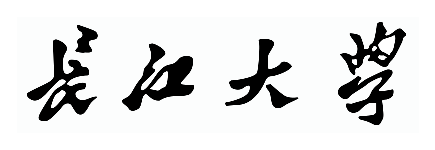
\includegraphics[width=3in]{pictures/yangtzeu.eps}}
    \centerline{������ѧ��������ҵ����LaTexģ��}
    \centerline{�����}
\end{titlepage}


% 目录
\newpage
\renewcommand{\contentsname}{\centerline{目录}}

\tableofcontents

% 示例章节 1
\section*{一、课程设计的目的}
\addcontentsline{toc}{section}{一、课程设计的目的}

恭承嘉惠兮,俟罪长沙\cite{lichangzhong2010jiyu}。侧闻屈原兮,自沉汩罗。造托湘流兮,敬吊先生。


% 示例章节 2
\section{��ѧ�½�}

����һ���ҵ���ѧ��ʽ\(\int_a^b f(x)dx\).�ž�����
    
��Ȼ,������������ʾ\[\int_a^b f(x)dx\]û�������Ƕ�ռһ��.




% 示例章节 3
\section{代码章节}

下面是一段代码:

\lstset{
	language=[ANSI]c,
	showspaces=false,
	escapeinside=``,
	breaklines,
	commentstyle=\color{red!50!green!50!blue!50},
	frame=shadowbox, 
	rulesepcolor=\color{red!20!green!20!blue!20},
	showstringspaces=false  % 字符串中显示空格
	}
	
\lstinputlisting{src/function.c}




% 参考文献
\newpage
\renewcommand\refname{\centerline{参考文献}}
\bibliographystyle{plain}
\bibliography{reference}


\end{CJK*}
\end{document}
